\documentclass[12pt]{article}
\usepackage{amsmath,amssymb,amsthm,bm}
\usepackage[usenames,dvipsnames]{xcolor}
\usepackage{graphicx}
%\usepackage{lmodern}
\usepackage[T1]{fontenc}
%\usepackage{textcomp}
\usepackage{pxfonts}
\usepackage{enumerate,verbatim,cite}
\usepackage[margin=1in]{geometry}
%\usepackage{../../tex/pythonhighlight} %https://github.com/olivierverdier/python-latex-highlighting

\usepackage{fancyhdr}
\pagestyle{fancy}
%\addtolength{\headheight}{\baselineskip}
\addtolength{\footskip}{\baselineskip}
\renewcommand{\headrulewidth}{0pt}
\renewcommand{\footrulewidth}{0.4pt}
\fancyhf{}
\fancyfoot[L]{\textit{Last Modified: \today}}
\fancyfoot[C]{\thepage}


\usepackage[pdftex,bookmarks,hyperfigures,colorlinks
						,urlcolor=blue
						,citecolor=blue
						,linkcolor=blue
						,pdfstartview=FitH]{hyperref}


%\usepackage{epsf}
% \topmargin -0.5in \setlength{\textwidth}{6.in}
% \setlength{\textheight}{8.5in}
%\setlength{\evensidemargin}{0.25in}
% \setlength{\oddsidemargin}{0.25in}
\renewcommand{\r}{{\bf r}}
\newcommand{\dery}{\frac{dx}{dt}}
\renewcommand{\k}{{\bf k}}
\newcommand{\be}{\begin{equation}}
\newcommand{\ee}{\end{equation}}
%\usepackage[usenames,dvipsnames]{xcolor}
%\usepackage{hyperref}

\newcommand{\myTitleBox}{
\noindent\makebox[\linewidth][c]{%
  %
    \parbox{\paperwidth}{%
      \hspace*{\dimexpr\hoffset+\oddsidemargin+1in\relax}%
      \begin{minipage}{\dimexpr\textwidth-2\fboxsep-2\fboxrule\relax}
      {\large\textbf{\courseTitleS}\courseTitle\hfill}\vspace{2mm}\\
%      {\large\textbf{\topicsCoveredS}\topicsCovered\hfill}\vspace{2mm}\\
      {\large\courseInstructors\hfill}\vspace{2mm}\\
%      \secAuthor\hfill\sectionTimesV\\
%      \authorContact\hfill\sectionTime\\
      \end{minipage}
    %
  }%
}
}


\newcommand{\courseTitleS}{CS109B/STAT121B/APCOMP209a/CSCI109B}
\newcommand{\courseTitle}{ Advanced Topics in Data Science}
\newcommand{\courseInstructors}{\textbf{Instructors:} Mark Glickman, Pavlos Protopapas}
%\newcommand{\sectionTimesV}{Section Times}
%\newcommand{\sectionTime}{ Wed 3-4pm \& Wed 5:30-6:30 \& Thurs 2:30-3:30}
%\newcommand{\topicsCoveredS}{Advanced Section 6:}
%\newcommand{\topicsCovered}{ Topics in Supervised Classification}
%\newcommand{\authorContact}{nhoernle@g.harvard.edu}
%\newcommand{\secAuthor}{Nick Hoernle}
\newcommand{\emptyS}{ }

%\title{\textbf{CS 109A Final Project} \\ \bigskip \large{Urban Crime Prediction}}
\date{}

\begin{document}
%\myTitleBox

\noindent {\small{\sc{CS 109B/Stat 121B/AC 209B/CSCI 109B: Final Project} \hfill \\ \small{\sc{Glickman, Protopapas}} \hfill \\ }
\begin{center}
\section*{Group 12\\Cancer Diagnosis in Medical Imaging}
\end{center}

%\maketitle

\subsection*{Literature Review}
\noindent For this project we will primarily be concerned with the work of Ronneberger, et al. [\ref{unet}]. In their paper \textit{U-Net: Convolutional Networks for Biomedical Image Segmentation}, Ronneberger, et al. focus on the design of a new network architecture, U-Net, which is a convolutional neural network designed for localization. Additionally, by utilizing data augmentation techniques, one can overcome the need for large amounts of training data, which is often not available in biomedical applications. 

\subsection*{Problem statement}
Finding suspicious nodules would typically be one of the first steps in identifying and treating lung cancer. This process can often be time-consuming given that after completing lung scans, the results need to be manually reviewed and annotated by a trained radiologist. The results of this review often require additional testing before making an official diagnosis. 

If the process of annotating and classifying lung nodules could be automated, physicians would be able to identify suspicious areas more quickly, thus speeding up the treatment and recovery of patients. 

In \textit{U-Net: Convolutional Networks for Biomedical Image Segmentation} [\ref{unet}], Ronneberger, et al. primarily focused the UNet architecture on applications relating to cell segmentation. We plan to expand this by applying UNet to the task of localization and annotation of lung nodules from diagnostic and lung cancer screening thoracic computed tomography (CT) scans. \\

\noindent \textbf{Project goal:} Train a UNet on data from the Lung Image Database Consortium image collection (LIDC-IDRI) [\ref{datalink}] to automate the annotation and classification of lung nodules.

\subsection*{Preliminary EDA}
\noindent  For this project we intend to use data from the Lung Image Database Consortium image collection [\ref{datalink}]. The dataset contains 244,527 images from 1,010 patients. Given the size of the dataset, using the entire set is likely impractical given resource and time constraints. However, one of the strong points of the UNet architecture, is that it can be trained on few images and still performs very well. Thus, we should be able to extract a more tractable size dataset and the network should still perform well. 

\begin{figure}
\centering
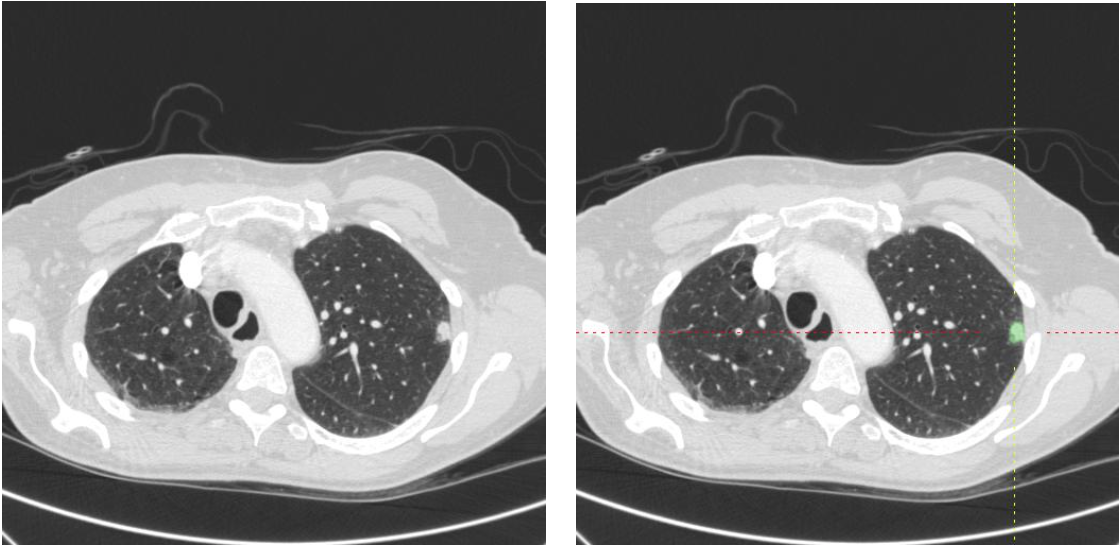
\includegraphics[width=.75\textwidth]{annotation_example}
\caption[width=.75\textwidth]{The image on the left is a raw image containing a nodule. In the image on the right, the nodule has been highlighted for clarity.}
\label{fig:img}
\end{figure}

In Figure~\ref{fig:img} you can see an example image. The image on the left is a raw image, while the image on the right has the annotated nodule highlighted for clairity. It should be noted that the annotations are encoded in an XML file, which will need to be extacted, and will only contain an outline (i.e. the border points) for each nodule. Below is a list of a few of the initial EDA work that will need to be completed. 

\begin{enumerate}
\item \textbf{Training and Test Data Extraction}\\
We will need to analyze the data available and extract appropriate test, training, and validation sets. This will require working with the available REST API to do this in an effecicient manner. 

\item \textbf{Extracting Annotations}
Once the data has been obtained, we will still face the problem of extracting the annonations. Each annotation is encoded in an XML file, which will need to be extracted and combined with the imaging data. 

\item \textbf{Data Exploration}
When the data is finally available for use, we will need to perform EDA on the image files to get a better idea of what types of data we will be working with, as well as data augmentation techniques. A few things we will need to consider:
\begin{itemize}
\item[-] Standardizing image sizes
\item[-] Standardizing image colors/channels
\item[-] Appropriate data augmentation techniques
\end{itemize} 
\end{enumerate}

\subsection*{References}
\begin{enumerate}
\item\label{datalink} \href{https://wiki.cancerimagingarchive.net/display/Public/LIDC-IDRI}{Lung Image Database Consortium image collection (LIDC-IDRI)} 

\item\label{unet} Ronneberger, O., Fischer, P., Brox, T.: U-Net: Convolutional Networks for Biomedical Image Segmentation (2015), arXiv:1505.04597 [cs.CV]
\end{enumerate}


\end{document}  